\Problem
{گام چهارم}
{
    با استفاده از دو دستور 
    \lr{imwrite} و \lr{imshow} 
    تصویر خاکستری شده را ذخیره می‌کنیم و نمایش می‌دهیم.
    
    \begin{figure}[H]
        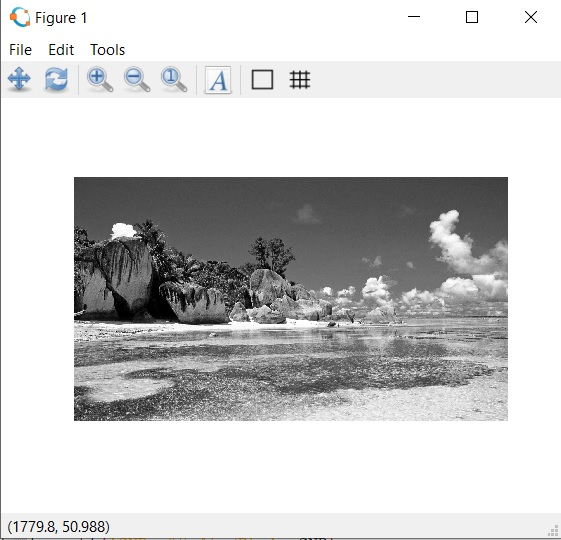
\includegraphics[width=13cm]{Images/imshow.jpg}
        \centering
        \caption{دستور \lr{imshow}}
    \end{figure}
    
    فرمت ذخیره‌سازی تصاویر را می‌توان در 3 دسته زیر تقسیم کرد:
    \begin{enumerate}
        \LTR
        \item \lr{Lossy compression}
        \item \lr{Lossless compression}
        \item \lr{Uncompressed}
    \end{enumerate}
    
    \RTL
    
    فرمت 
    \lr{JPG} 
    از نوع اول می‌باشد و هنگام فشرده‌سازی بخشی از اطلاعات عکس حذف می‌شوند و دیگر قابل برگشت نیستند. این تصاویر دارای حجم کمتری هستند و مناسب دنیای اینترنت هستند.
    
    فرمت 
    \lr{PNG} 
    از نوع دوم می‌باشد و هنگام فشرده‌سازی اطلاعاتی از دست نمی‌دهد و می‌توان تصویر فشرده شده را به تصویر اولیه برگرداند. بنابراین حجم بیشتری نسبت به حالت بالا دارد.
    
    فرمت 
    \lr{BMP} 
    از نوع سوم می‌باشد و هنگام ذخیره‌سازی هیچ فشرده‌سازی انجام نمی‌دهد. حجم تصاویر در این حالت بسیار بالا بوده زیرا تمامی جزئیات و اطلاعات تصویر در این فرمت حفظ و ذخیره می‌شود. البته در بعضی حالت‌های این فرمت می‌توان فشرده‌سازی نیز داشت. فرمت ذخیره‌سازی 
    \lr{TIFF} 
    نیز از همین نوع می‌باشد.
    
    نکته: برای کاهش حجم پروژه ارسالی تصاویر را در حالت \lr{JPG} ذخیره کردیم. اما حالت بدون فشرده‌سازی \lr{BMP} است.
    
}
